\section{Diseño (Desarrollo Teórico )}
\subsection{Diagrama a bloques del sistema}
En la siguiente figura, se muestra el diagrama a bloques del sistema, donde se destaca que es lo que
conforma cada una de las partes de potencia, microprocesador, comunicacion y perifericos.
\begin{figure}[htp]
    \centering
    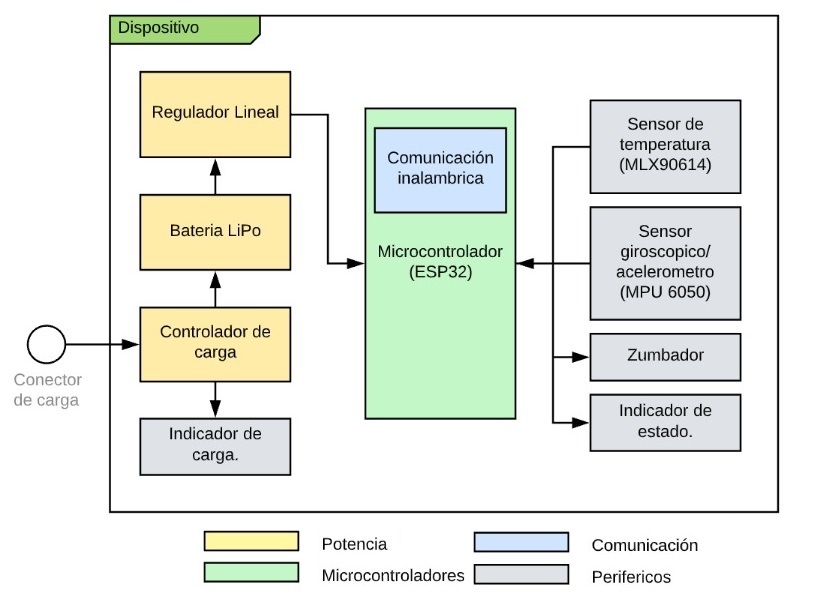
\includegraphics[width=\columnwidth]{system_block_diagram.png}
    \caption{Diagrama a bloques del sistema}
\end{figure}

\subsection{ESP32}
ESP32 es la denominación de una familia de chips SoC de bajo costo y consumo de energía, con tecnología Wi-Fi y Bluetooth de modo dual integrada. El ESP32 emplea un microprocesador Tensilica Xtensa LX6 en sus variantes de simple y doble núcleo e incluye interruptores de antena, balun de radiofrecuencia, amplificador de potencia, amplificador receptor de bajo ruido, filtros, y módulos de administración de energía. El ESP32 fue creado y desarrollado por Espressif Systems y es fabricado por TSMC utilizando su proceso de 40 nm.

\textbf{Características}
\begin{itemize}
    \item Procesador:
          \begin{itemize}
              \item CPU: microprocesador de 32-bit Xtensa LX6 de doble núcleo (o de un solo núcleo), operando a 160 o 240 MHz y rindiendo hasta 600 DMIPS.
              \item Co-procesador de ultra baja energía (ULP).
          \end{itemize}
    \item Memoria: 520 KiB SRAM
    \item Conectividad inalámbrica:
          \begin{itemize}
              \item Wi-Fi: 802.11 b/g/n
              \item Bluetooth: v4.2 BR/EDR y BLE
          \end{itemize}
    \item Interfaces periféricas:
          \begin{itemize}
              \item 12-bit SAR ADC de hasta 18 canales
              \item 2 × 8-bit DACs
              \item 10 × sensores de tacto (sensores capacitivos GPIOs)
              \item 4 × SPI
              \item 2 × interfaces I²S
              \item 2 × interfaces I²C
              \item 3 × UART
              \item Controlador host SD/SDIO/CE-ATA/MMC/eMMC
              \item Controlador esclavo SDIO/SPI
              \item Interfaz Ethernet MAC con DMA dedicado y soporte para el protocolo IEEE 1588 Precision Time Protocol
              \item Bus CAN 2.0
              \item Controlador remoto infrarrojo (TX/RX, hasta 8 canales)
              \item Motor PWM
              \item LED PWM (hasta 16 canales)
              \item Sensor de efecto Hall
              \item Pre-amplificador analógico de ultra baja potencia
          \end{itemize}
    \item Seguridad:
          \begin{itemize}
              \item Soporta todas las características de seguridad estándar de IEEE 802.11, incluyendo WFA, WPA/WPA2 y WAPI
              \item Arranque seguro
              \item Cifrado flash
              \item 1024-bit OTP, hasta 768-bit para clientes
              \item Criptografía acelerada por hardware: AES, SHA-2, RSA, criptografía de curva elíptica (ECC), generador de números aleatorios (RNG)
          \end{itemize}
    \item Administración de energía:
          \begin{itemize}
              \item Regulador interno de baja caída
              \item Dominio de poder individual para RTC
              \item Corriente de 5microA en modo de suspensión profundo
              \item Despierta por interrupción de GPIO, temporizador, medidas de ADC, interrupción por sensor de tacto capacitivo
          \end{itemize}
\end{itemize}

\textbf{Uso}

El monitoreo en el Sistema de Prevención para la muerte de lactantes es crítico y es necesario de un MPU que sea capaz de realizar operaciones aritméticas lo más eficiente posible y al tener un procesador operando a 160 o 240 MHz y rindiendo hasta 600 DMIPS.

Así mismo El ESP32 cuenta módulos de comunicación tanto de bluetooth y wifi, lo que hace nuestro sistema más compacto y así no sea evasivo con el lactante porque utilizamos menos componentes.

Las interfaces I²C facilitan la comunicación entre los sensores al ser la transferencia de datos es siempre inicializada por un maestro; el esclavo reacciona. Esto hace posible tener varios maestros mediante un modo multimaestro, en el que se pueden comunicar dos maestros entre sí, de modo que uno de ellos trabaja como esclavo.

El bajo consumo de energía hace que la batería de litio de 3.6v que se implementa en el sistema duré un promedio de 16hrs lo cual es un tiempo razonable para el monitoreo del sueño del lactante.
\begin{figure}[htp!]
    \centering
    \includegraphics[width=\columnwidth]{ESP32.jpg}
    \caption{ESP32}
    \label{fig: esp32}
\end{figure}\FloatBarrier
\subsection{Sensores}
\textbf{MPU-9250}

El MPU-9250 de InvenSense, es un dispositivo de medicion inercial (IMU) de 9 ejes, que combina un giroscopio de 3 ejes,
un acelerómetro de 3 ejes, y un magnetómetro de 3 ejes, donde cada uno de estos cuenta con:
\begin{itemize}
    \item Tres convertidores analógico-digitales (ADC) de 16 bits para digitalizar sus salidas.
    \item Registros individuales de configuración, ya sea para rangos, frecuencia de muestreo, habilitación, etc.
\end{itemize}

La union de estos tres sensores y sus posibles configuraciones permiten el desarrollo de sistemas de deteccion/medicion de
movimientos con una buena fiabilidad.

\begin{figure}[htp]
    \centering
    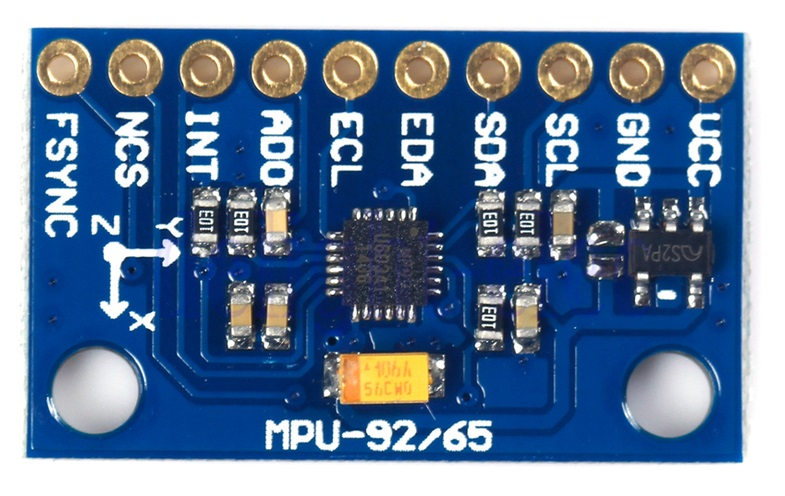
\includegraphics[width=5cm]{mpu_9250_board.png}
    \caption{MPU-9250 }
\end{figure}

\textbf{Caracteristicas}

\begin{itemize}
    \item Giroscopio de tres ejes de salida digital con un rango de escala completa programable de $ \pm $250, $ \pm $500, $ \pm $1000 y $ \pm $2000°/seg.
    \item Acelerómetro de tres ejes de salida digital con un rango de escala completa programable de $ \pm $2g, $ \pm $4g, $ \pm $8g y $ \pm $16g.
    \item Sensor magnético monolítico de efecto Hall de 3 ejes con concentrador magnético con resolucion de 0,6T/LSB.
    \item Cuenta con interfaz para comunicacion por SPI y I2C.
\end{itemize}

\textbf{Sensor de temperatura infrarrojo MLX90614}

El Sensor de temperatura infrarrojo permite medir la temperatura de un objeto a distancia (sin contacto). El Sensor MLX90614 es un chip de silicio con una fina membrana micro mecanizada, diseñada para ser sensible a la radiación infrarroja emitida por un objeto a distancia. El sensor posee internamente una etapa de amplificación y digitalización (ADC) de la señal procedente de la membrana. La salida del sensor es lineal y se compensa de acuerdo con las variaciones de la temperatura ambiente.

El sensor MLX90614 integra un circuito de filtrado de ruido, un conversor A/D(ADC) de 17 bits de resolución y un procesador digital de señales, entregando un amplio rango de trabajo para objetos desde -70°C hasta 380°C, con una precisión de 0.5°C.

La salida del sensor es una interfaz de comunicación digital tipo SMBus, que es un subconjunto del protocolo I2C. El sensor permite además configurar una salida PWM de 10 bits.

\textbf{Especificaciones Técnicas}
\begin{itemize}
    \item Módulo: GY-906
    \item Chip sensor: MLX90614ESF-BAA
    \item Voltaje de operación: 3.3V-5V DC
    \item Protocolo de comunicación SMBUS (subconjunto del I2C)
          %\item Rango de temperatura ambiente de trabajo: -40$\circ$C hasta +170℃
          %\item Rango de temperatura de objeto: -70℃ hasta +380℃
    \item Precisión: $ \pm $0.5°C
    \item ADC interno de 17 bits
    \item Procesador digital de señal interno
    \item Regulador de voltaje 3.3V en placa
    \item Resistencias Pull-up a VIN en placa
    \item No necesita componentes adicionales
    \item Dimensiones: 16*11*6 mm
    \item Peso: 2.80 gramos
    \item Conexión
          \begin{itemize}
              \item VIN: +3.3V - +5.0V DC
              \item GND: 0V Tierra
              \item SCL: I2C clock
              \item SDA: I2C data
          \end{itemize}
\end{itemize}
\begin{figure}[htp!]
    \centering
    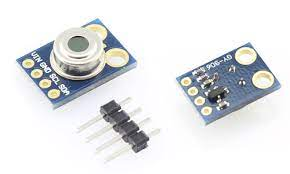
\includegraphics[width=\columnwidth]{sensor_MLX90614.jpg}
    \caption{Sensor MLX90614}
    \label{fig: sensor}
\end{figure}\FloatBarrier
\textbf{Ejemplos de aplicación}
\begin{itemize}
    \item Sensor de confort térmico para Mobile Air
    \item Sistema de control de acondicionamiento
    \item Elemento sensor de temperatura para residencial, comercial e industrial
    \item Desempañado de parabrisas
    \item Detección de ángulo muerto automotriz
    \item Control de temperatura industrial de movimiento partes
    \item Control de temperatura en impresoras y fotocopiadoras
    \item Electrodomésticos con control de temperatura
    \item Salud
    \item Monitoreo de ganado
    \item Detección de movimiento
    \item Control de temperatura de múltiples zonas
    \item Relé térmico / alerta
    \item Medición de la temperatura corporal
\end{itemize}

\subsection{Bluetooth Low Energy}
Es una tecnología de red de área personal inalámbrica, diseñada y comercializada por Bluetooth SIG destinada a aplicaciones en el cuidado de la salud, fitness y beacons,1 seguridad y las industrias de entretenimiento en el hogar Comparado con Bluetooth clásico, Bluetooth Low Energy está diseñado para proporcionar un bajo consumo de energía, manteniendo un rango de alcance de comunicación similar.

Los sistemas operativos móviles, incluidos iOS, Android, Windows Phone y BlackBerry, así como macOS, Linux, Windows 8 y Windows 10, son compatibles con Bluetooth Low Energy. Bluetooth SIG predice que el 100\% de los dispositivos con Bluetooth comercializados hasta 2024 soportaran Bluetooth Low Energy.

\textbf{Características}

\begin{itemize}
    \item Permite la comunicación entre dispositivos de pila de botón y dispositivos.
    \item Bluetooth, que opera en 2.4 GHz (una de las bandas ISM), con una tasa de transferencia de 1 Mbps en la capa física.
    \item Los chips de BLE tienen amplias opciones de empleo en la industria.
    \item Tienen el mismo tamaño de los dispositivos Bluetooth clásicos.
    \item Tiene soporte para seguridad, ya que emplean el sistema de cifrado AES y esquemas de seguridad configurables.

\end{itemize}

\begin{figure}[htp!]
    \centering
    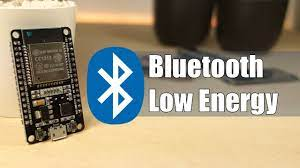
\includegraphics[width=\columnwidth]{bluetooth.jpg}
    \caption{Bluetooth BLE y ESP32}
    \label{fig: Bluetooth}
\end{figure}\FloatBarrier

